
% !TEX TS-program = xelatex
% !TEX encoding = UTF-8 Unicode

% \documentclass[AutoFakeBold]{LZUThesis}
\documentclass[AutoFakeBold]{LZUThesis}

\begin{document}
%=====%
%
%封皮页填写内容
%
%=====%

% 标题样式 使用 \title{{}}; 使用时必须保证至少两个外侧括号
%  如: 短标题 \title{{第一行}},  
% 	      长标题 \title{{第一行}{第二行}}
%             超长标题\tiitle{{第一行}{...}{第N行}}

\title{{人类ABO血型和部分单基因性状的遗传分析}}



% 标题样式 使用 \entitle{{}}; 使用时必须保证至少两个外侧括号
%  如: 短标题 \entitle{{First row}},  
% 	      长标题 \entitle{{First row}{ Second row}}
%             超长标题\entitle{{First row}{...}{ Next N row}}
% 注意:  英文标题多行时 需要在开头加个空格 防止摘要标题处英语单词粘连。
\entitle{{Genetic Analysis of Human ABO Blood Types and Some Monogenic Traits}}

\author{生物信息学班 李泽华 320210928501}
\major{遗传学}
\advisor{王铭裕}
\college{生命科学学院}
\grade{2021级}



%\maketitle

%==============================%
% ↓ ↓ ↓ 诚信说明页 授权说明书
%==============================%

% 1. 可以调整签字的宽度,现在是40
% 2. 去掉raisebox的相关注释(注意上下大括号对应),可以改变-5那个数字调整签名和横线的上下位置

% 你的签名,signature.pdf 改为你的签名文件名,
\mysignature{
    % \raisebox{-5pt}{
    
\includegraphics[width=40pt]{signature.pdf}
    % }
}
% 你手写的日期,signature.pdf 改为你的手写的日期文件名
\mytime{
    % \raisebox{-5pt}{
    
\includegraphics[width=40pt]{signature.pdf}
    % }
}
% 老师的手写签名,signature.pdf 改为老师的手写签名文件名
\supervisorsignature{
    % \raisebox{-5pt}{
    
\includegraphics[width=40pt]{signature.pdf}
    % }
}
% 老师手写的时间,signature.pdf 改为老师的手写的日期文件名
\teachertime{
    % \raisebox{-5pSt}{
    
\includegraphics[width=40pt]{signature.pdf}
    % }
}
% 老师手写的成绩
\recommendedgrade{
    % \raisebox{-5pt}{
    
\includegraphics[width=40pt]{signature.pdf}
    % }
}

%\makestatement

%==============================%
% ↑ ↑ ↑ 诚信说明页 授权说明书
%==============================%


%=====%
%论文(设计)成绩:注意2007的模板要求,成绩页在最后,2021要求成绩页在摘要前面
%=====%

%% 下面这些注释掉可以去掉成绩、评语什么的
%\supervisorcomment{导师评价你人很好}
%
%
%\committeecomment{优秀}
%
%\finalgrade{100}
%% 上面这些注释掉可以去掉成绩、评语什么的


\frontmatter



%中文摘要
\ZhAbstract{
    本实验通过对兰州大学21级生命科学学院学生的ABO血型进行调查分析,深入探讨了基因在群体水平上的传递规律。通过统计数据,
    计算基因频率和基因型频率,利用Hardy-Weinberg平衡定律进行群体遗传结构分析。结果显示,在该群体中,O型血的频率最高,其次为A型血和B型血,而AB型血的频率最低。经过基因型频率的统计和卡方检验,发现群体处于遗传平衡状态。这一研究有助于增进对基因在人群中的遗传规律的理解,为进一步研究遗传学提供了基础。
}{ABO血型,遗传平衡,基因频率,基因型频率,Hardy-Weinberg平衡定律,群体遗传结构分析}


%英文摘要
\EnAbstract{
    This experiment investigates and analyzes the ABO blood types of students from the 2021 class at the School of Life Sciences, Lanzhou University, aiming to explore the transmission patterns of genes at the population level. Through data collection, gene frequency, and genotype frequency calculations, the study employs the Hardy-Weinberg equilibrium law for population genetic structure analysis. The results reveal that in this population, blood type O has the highest frequency, followed by blood types A and B, with blood type AB having the lowest frequency. Statistical analysis of genotype frequency and chi-square tests indicate that the population is in genetic equilibrium. This research contributes to a better understanding of the genetic patterns in populations, providing a foundation for further genetic studies.
}{ABO blood type, genetic equilibrium, gene frequency, genotype frequency, Hardy-Weinberg equilibrium law, population genetic structure analysis}

%生成目录
% \tableofcontents
% 下面这个包含图表目录
\customcontent


% % 部分同学需要专业术语注释表,* 表示不加入目录
% \chapter*{专业术语注释表}
% \begin{longtable}{lll}
%   \caption*{缩略词说明}\\
%   SS & Spread Spectrum & 扩展频谱 \\
%   PAPR & Peak to Average Power Ratio & 峰均比\\
%   DCSK & Differential Chaos Shift Keying &差分混移位键控\\
%   dasd & fdhfudw eqwrqw fasfasfs fewev wqfwefew &\tabincell{l}{太长了\\换行一下}\\
% \end{longtable}


%文章主体
\mainmatter

\chapter{\texorpdfstring{绪 \quad 论}{绪论}}

% !学校要求的规范,绪论是单独的,不是第一章,但是老师们都是让作为第一章,这里我把它放在了论文里,如果你要让在外面,只需要把上面的 \mainmatter 这一句话放在“绪论内容后面,正文第一章前面”即可,也就是 \chapter{latex部分用法简介} 这一句话上面
遗传学是生物学的一个重要分支,研究基因在生物体遗传过程中的传递规律和变异现象。通过对基因的调查和分析,人们可以更深入地了解群体的遗传结构、基因频率以及基因型频率等重要信息。本实验旨在通过对人类ABO血型和部分单基因性状的遗传分析,深入探讨基因在群体水平上的传递规律,掌握基因频率和基因型频率的估算方法,并进一步理解Hardy-Weinberg平衡定律及其影响因素。

首先,通过对ABO血型的调查分析,我们可以了解基因在群体中的传递规律。ABO血型是人类最早认知的血型系统之一,其遗传基础由三个主要等位基因决定,分别为IA(A)、IB(B)和i(O)。通过调查血型数据,我们可以推测基因型频率和基因频率,并使用Hardy-Weinberg平衡定律对群体进行遗传学分析。这有助于我们更好地理解基因在群体中的平衡状态,以及可能影响平衡的因素。

其次,通过调查人类部分单基因性状,我们将观察和统计不同性状在群体中的频率。这些性状包括耳垂类型、舌卷类型、眼睑形态等,它们由单个基因控制,并在群体中呈现出特定的遗传规律。我们将利用系谱分析法对这些性状进行调查,以初步了解它们的遗传特性,并通过统计数据进行群体遗传结构分析。

通过这次实验,我们旨在培养对遗传学的实际操作能力,深入了解人类基因的遗传规律,并通过数据分析和统计推断群体的遗传状态。这对于培养实验技能、科学思维和数据分析能力具有重要意义。

% TODO 正文。是毕业论文(设计)的核心部分,包括研究背景、立论根据、研究内容、研究方法与过程、研究结果与分析、研究结论及其意义。要求论述正确、逻辑严密、层次分明、文字流畅简练、公式图表清晰规范、数据真实可靠,公式推导和计算结果正确无误。毕业论文(设计)中如出现非通用性新名词、新术语、新概念,应作相应解释。

\chapter{研究背景}

\section{Hardy-Weinberg平衡定律}
也称遗传平衡定律或哈代-温伯格平衡定律\cite{WOS:000258376000019}},分别在1908年和1909年由英国数学家戈弗雷·哈罗德·哈代和德国医生威廉·温伯格独立证明。
在群体遗传学中,哈代-温伯格定律主要用于描述群体中等位基因频率以及基因型频率之间的关系。主要内容为:
\begin{quote}
{\bfseries\fangsong 一个族群在理想情况(不受特定的干扰因素影响,如非随机交配、天择、族群迁移、突变或群体大小有限), 经过多个世代,基因频率与基因型频率会保持恒定并处于稳定的平衡状态}
\end{quote}

\begin{figure}[H]
    \centering
    \subfloat[ardy-Weinberg平衡定律]{
        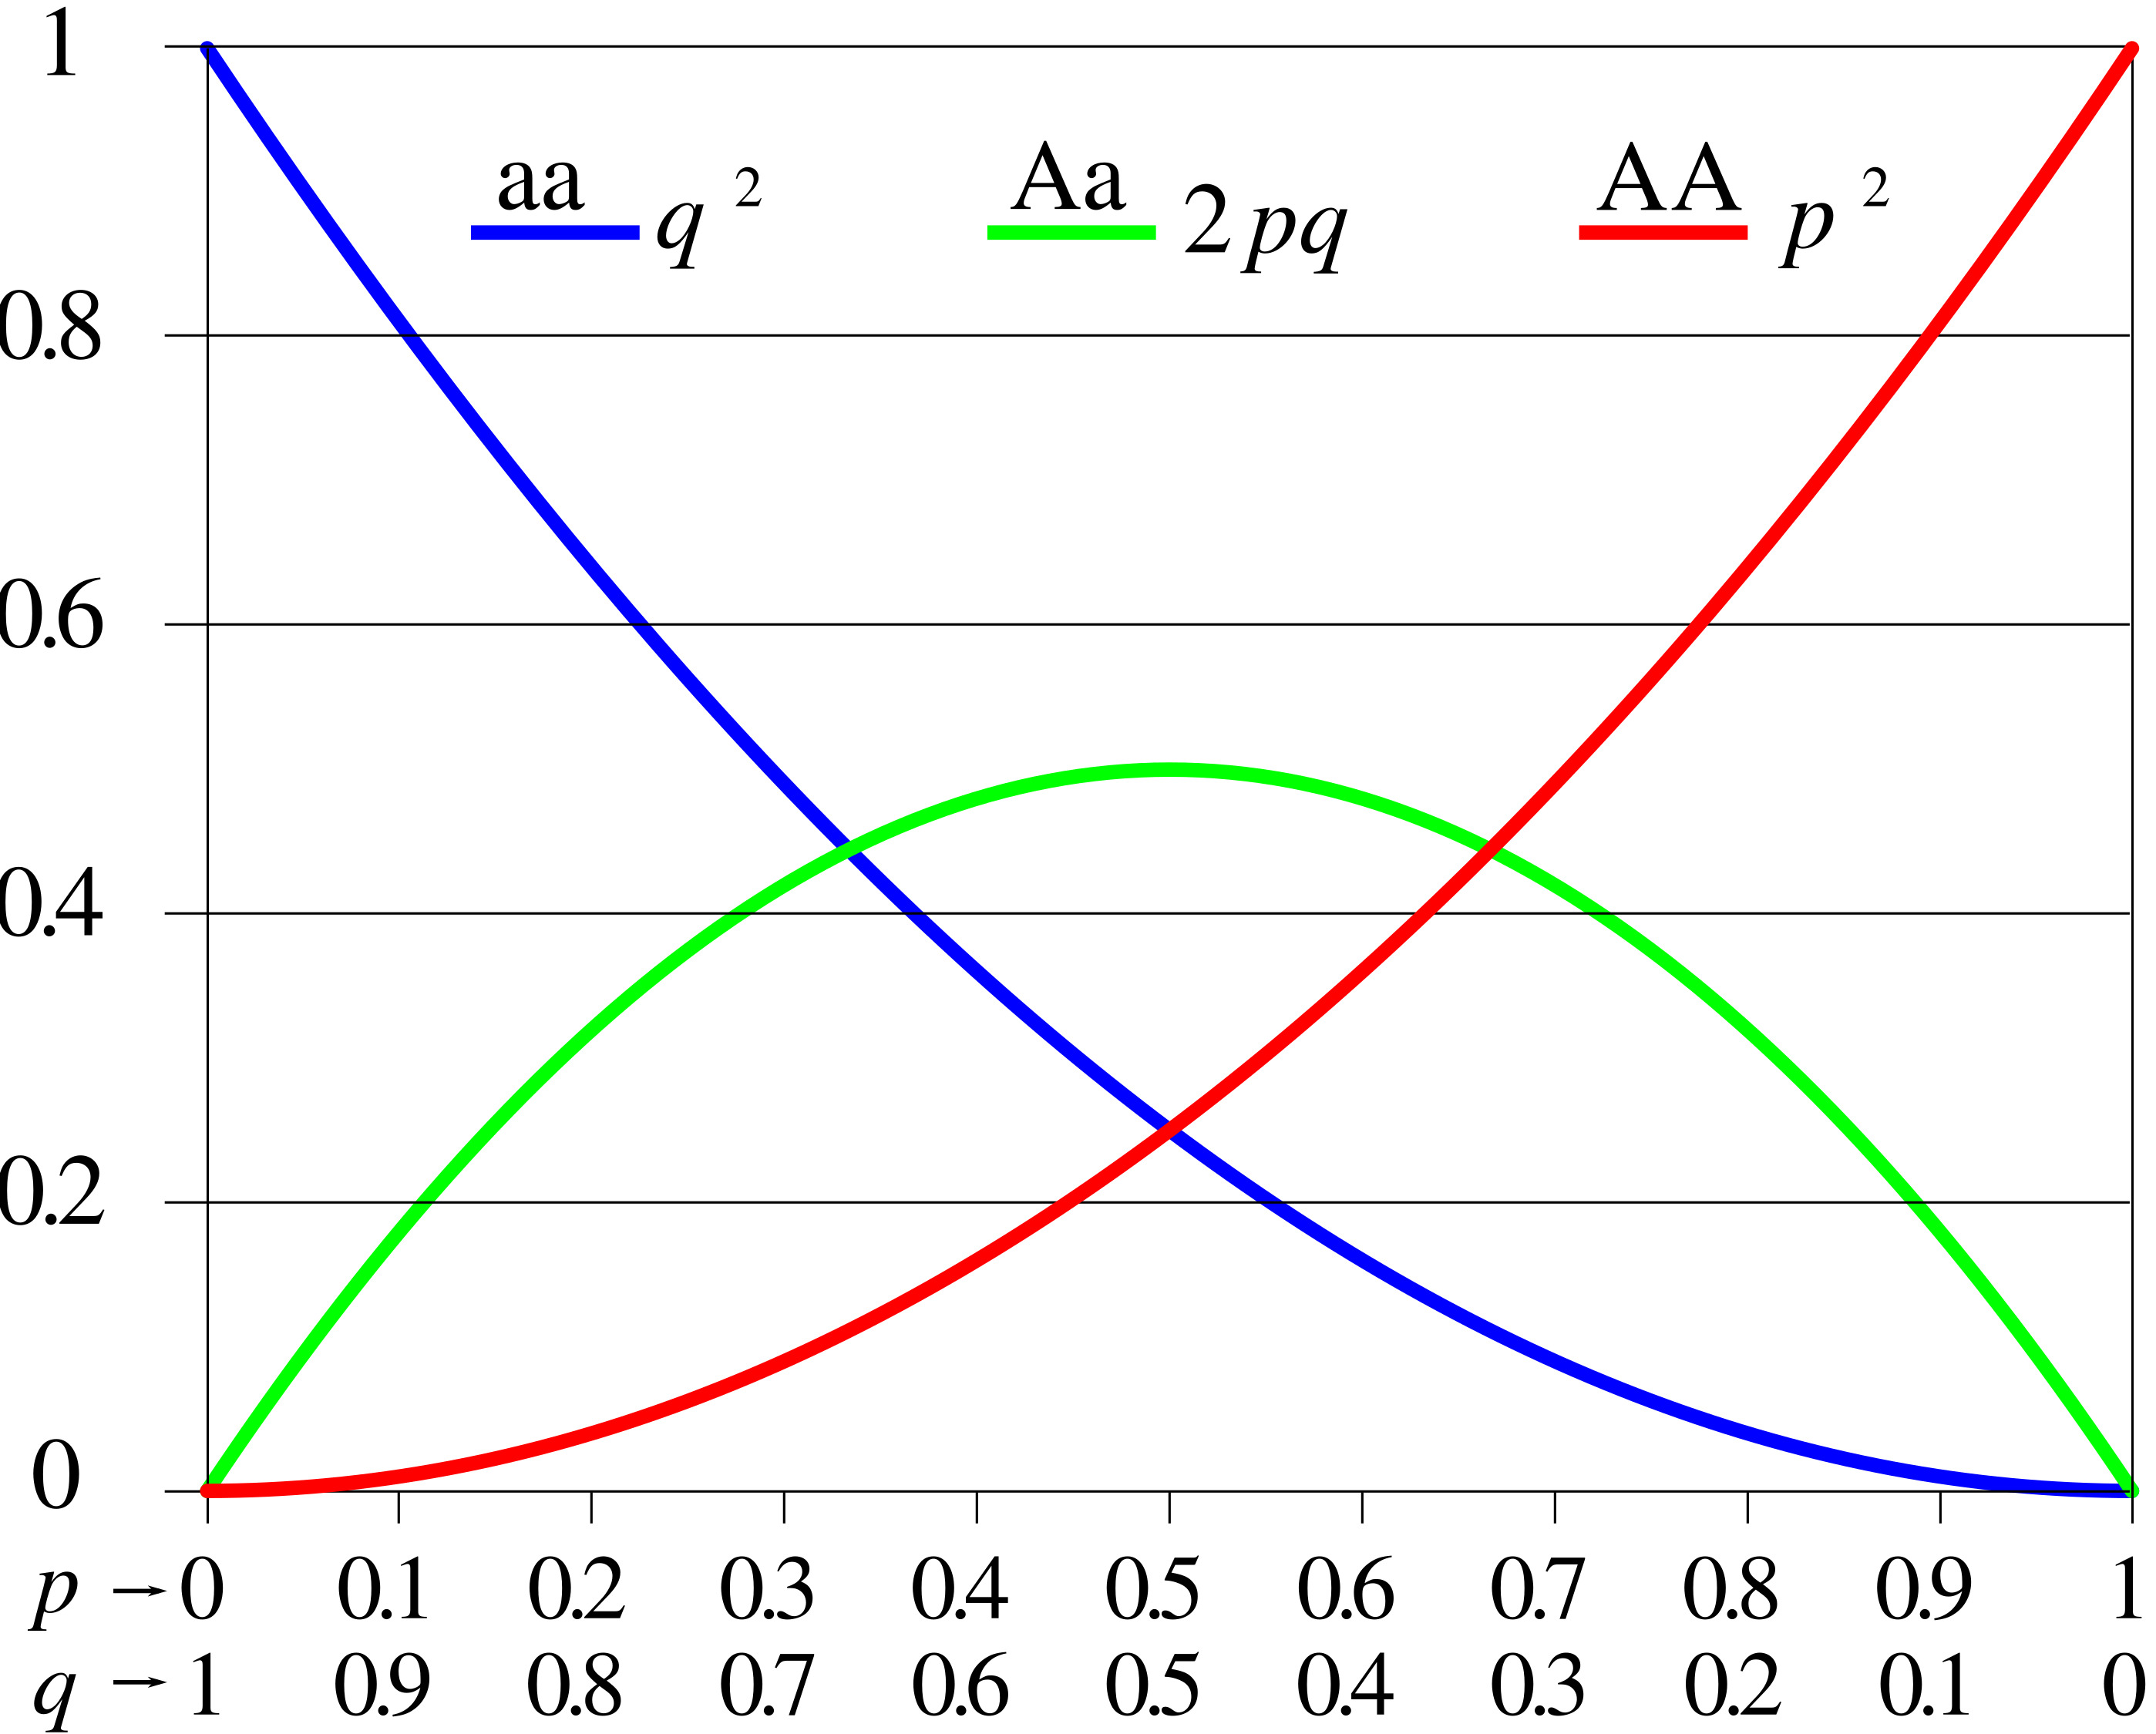
\includegraphics[width=150pt]{./img/Hardy-Weinberg}
    }
    \caption{对于两个等位基因的哈代-温伯格定律: 横轴表示两个等位基因频率p和q,而纵轴表示基因型频率。每条线表示一种基因型频率。我们假设纵切穿过三线,形成三个点,在一个极为稳定的族群中比值亦该相当类似三点的比值。}
    \label{fig_ldr}
\end{figure}


在实际应用中, 符合理想条件的群体一般不存在, 但对Hardy-Weinberg平衡定律的影响不大, 因为我们所调查的群体不可能足够大到显示出这些影响因素

\section{人类ABO血型的群体遗传分析}
\begin{itemize}
    \item 历史\par
    1900年,奥地利维也纳大学病理研究所的生物学家卡尔·兰德施泰纳首次报道,健康人的血清对一些人类个体的红细胞有凝聚作用。通过混合不同人的血清和红细胞,他发现了A、B、O三种血型,他的学生Alfred von Decastello和Sturli又于两年后发现了第四种——AB型. 兰德施泰纳因此获得1930年度诺贝尔生理学或医学奖。

    \item ABO抗原\par
    编码ABO抗原决定簇的是9号染色体上的ABO基因,总长度18000至20000个碱基对,包括7个外显子,其中最大的第7外显子和第6外显子的碱基数占整个编码序列的77%.
    ABO基因有三个最主要的等位基因:IA(A)、IB(B)和i(O),这些等位基因的原初产物是糖基转移酶。IA等位基因编码α-1,3N-乙酰氨基半乳糖转移酶,
    能将α-N-乙酰半乳糖胺接到H抗原的β-D-半乳糖上,形成A抗原;IB等位基因编码α-1,3-D-半乳糖转移酶,将α-D-半乳糖接到H抗原的相同位置,形成B抗原;
    i等位基因的第6外显子包含一个核苷酸缺失,导致其编码的蛋白质无法正常表达,从而失去酶活性,因此,O型血的抗原就是未经改变的H抗原。

    \begin{longtable}{cccc}
        \toprule
        血型 & 基因型 & 红细胞膜上的抗原 & 血清中的抗体 \\
        \midrule
        A & I\textsuperscript{A}I\textsuperscript{A}, I\textsuperscript{A}i & A & 抗B($\beta$) \\
        B & I\textsuperscript{B}I\textsuperscript{B}, I\textsuperscript{A}i & B & 抗A($\alpha$) \\
        O & ii & NULL & 抗A($\alpha$) OR 抗B($\beta$) \\
        AB & I\textsuperscript{A}I\textsuperscript{B} & A \& B & NULL \\
        \bottomrule
        \caption{ABO血型系统}
    \end{longtable}
    \item 抗原检测\par
    在鉴定人的血型时,既要用标准的抗A和抗B血清鉴定被检者红细胞上的抗原(直接试验法),同时要用标准的A型和B
    型红细胞鉴定被检者血清中的抗体(反转试验法)。只有被检者红细胞上的抗原鉴定和血清中的抗体鉴定所得结果完全相符时才能确定其血型类别。实验室一般采用直接试验法。
    对于不知血型者或自愿者,可以采用玻片法进行血型检测,然后通过统计、分析,就可估算出AB0血型的基因频率和基因型频率。

    \item 人类血型系统\par
    人类红细胞膜表面各种血型抗原系统的统称。根据国际输血协会(International Society of Blood
    Transfusion,ISBT)的认定,包括最为常见的ABO血型系统和恒河猴血型系统(Rh)在内,共有30种主要血型系统。
\end{itemize}

\begin{longtable}{p{1.cm}p{2cm}cp{1.5cm}cp{3cm}}
    \toprule
    \textbf{ISBT编号} & \textbf{中文名称} & \textbf{英文简称} & \textbf{编码基因名称} & \textbf{编码基因位置} & \textbf{抗原决定基团类型/备注} \\
    \midrule
    001 & \small ABO血型系统 & ABO & \textit{ABO} & 9q34.2 & \tiny 寡聚糖,不同的等位基因编码不同的糖基转移酶,其基础是Hh血型系统;ABO血型系统是人类最早认识和最为重要的血型系统 \\
    002 & \small MNS血型系统 & MNS & \textit{GYPA}\newline\textit{GYPB}\newline\textit{GYPE} & 4q31.21 & \tiny GPA/GPB(血型糖蛋白A和B),主要抗原:M、N、S、s \\
    003 & \small P血型系统 & P1 & & 22q11.2–qter & 糖脂 \\
    004 & \small Rh血型系统 & RH & \textit{RHD}\newline\textit{RHCE} & 1p36.11 & \tiny 蛋白质:C、c、D、E、e抗原(不存在“d”抗原; “d”代表无D抗原)。是在医学上占有第二位重要意义的血型系统 \\
    005 & \small Lutheran血型系统 & LU & \textit{LU} & 19q13.32 & \tiny 蛋白质(免疫球蛋白超家族的成员),已发现21种抗原 \\
    006 & \small Kell血型系统 & KEL & \textit{KEL} & 7q34 & \tiny 糖蛋白,K₁可能引起严重新生儿溶血症(抗-Kell型) \\
    007 & \small Lewis血型系统 & LE & \textit{FUT3} & 19p13.3 & \tiny 糖类(岩藻糖片段,主要抗原:Le\textsuperscript{a}与Le\textsuperscript{b},与ABH抗原分泌有关 \\
    008 & \small Duffy血型系统 & FY & \textit{DARC} & 1q23.2 & \tiny 糖蛋白,为趋化因子受体(chemokine receptor),主要抗原Fy\textsuperscript{a}和 Fy\textsuperscript{b},缺乏Duffy抗原者对间日疟原虫(*Plasmodium vivax*)和诺氏疟原虫(*Plasmodium knowlesi*)引起的疟疾免疫 \\
    009 & \small Kidd血型系统 & JK & \textit{SLC14A1} & 18q12.3 & \tiny 蛋白质(尿素通道蛋白),主要抗原:Jk\textsuperscript{a}和 Jk\textsuperscript{b} \\
    010 & \small Diego血型系统 & DI & \textit{SLC4A1} & 17q21.31 & \tiny 糖蛋白/ 糖蛋白(Glycoproteins)(红细胞膜带3蛋白),阳性个体只存在于东亚人群和印第安人中 \\
    011 & \small Yt血型系统 & YT & \textit{ACHE} & 7q22.1 & \tiny 蛋白质,即乙酰胆碱酯酶(AChE) \\
    012 & \small XG血型系统 & XG & \textit{XG}\newline\textit{MIC2} & Xp22.33 & 糖蛋白 \\
    013 & \small Scianna血型系统 & SC & \textit{ERMAP} & 1p34.2 & 糖蛋白 \\
    014 & \small Dombrock血型系统 & DO & \textit{ART4} & 12p12.3 & \tiny 糖蛋白(由GPI固定于细胞膜上),或称糖基化磷脂酰肌醇(glycosyl-phosphatidyl-inositol,GPI)锚定蛋白 \\
    015 & ... & ... & ... & ... & ... \\
    \bottomrule
    \caption{人类血型系统信息表格}
\end{longtable}

\begin{itemize}
    \item 中国人群ABO血型分布\par
\end{itemize}

根据陕西省人民医院大数据统计的结果\cite{WOS:000879413200018}
\begin{enumerate}
    \item 中国人ABO血型分布特征为O>A>B>AB,中国1441497378人口,O型人数最多为492986063人,占34.20\%,
    A型人数次之为414019735人,占28.72\%,B型血人数为406034740,占28.17\%,
    AB型人数最少为128456841人,占8.91\%。(见图\ref{fig:ChinaABO-1})

    \begin{figure}[H]
        \centering
        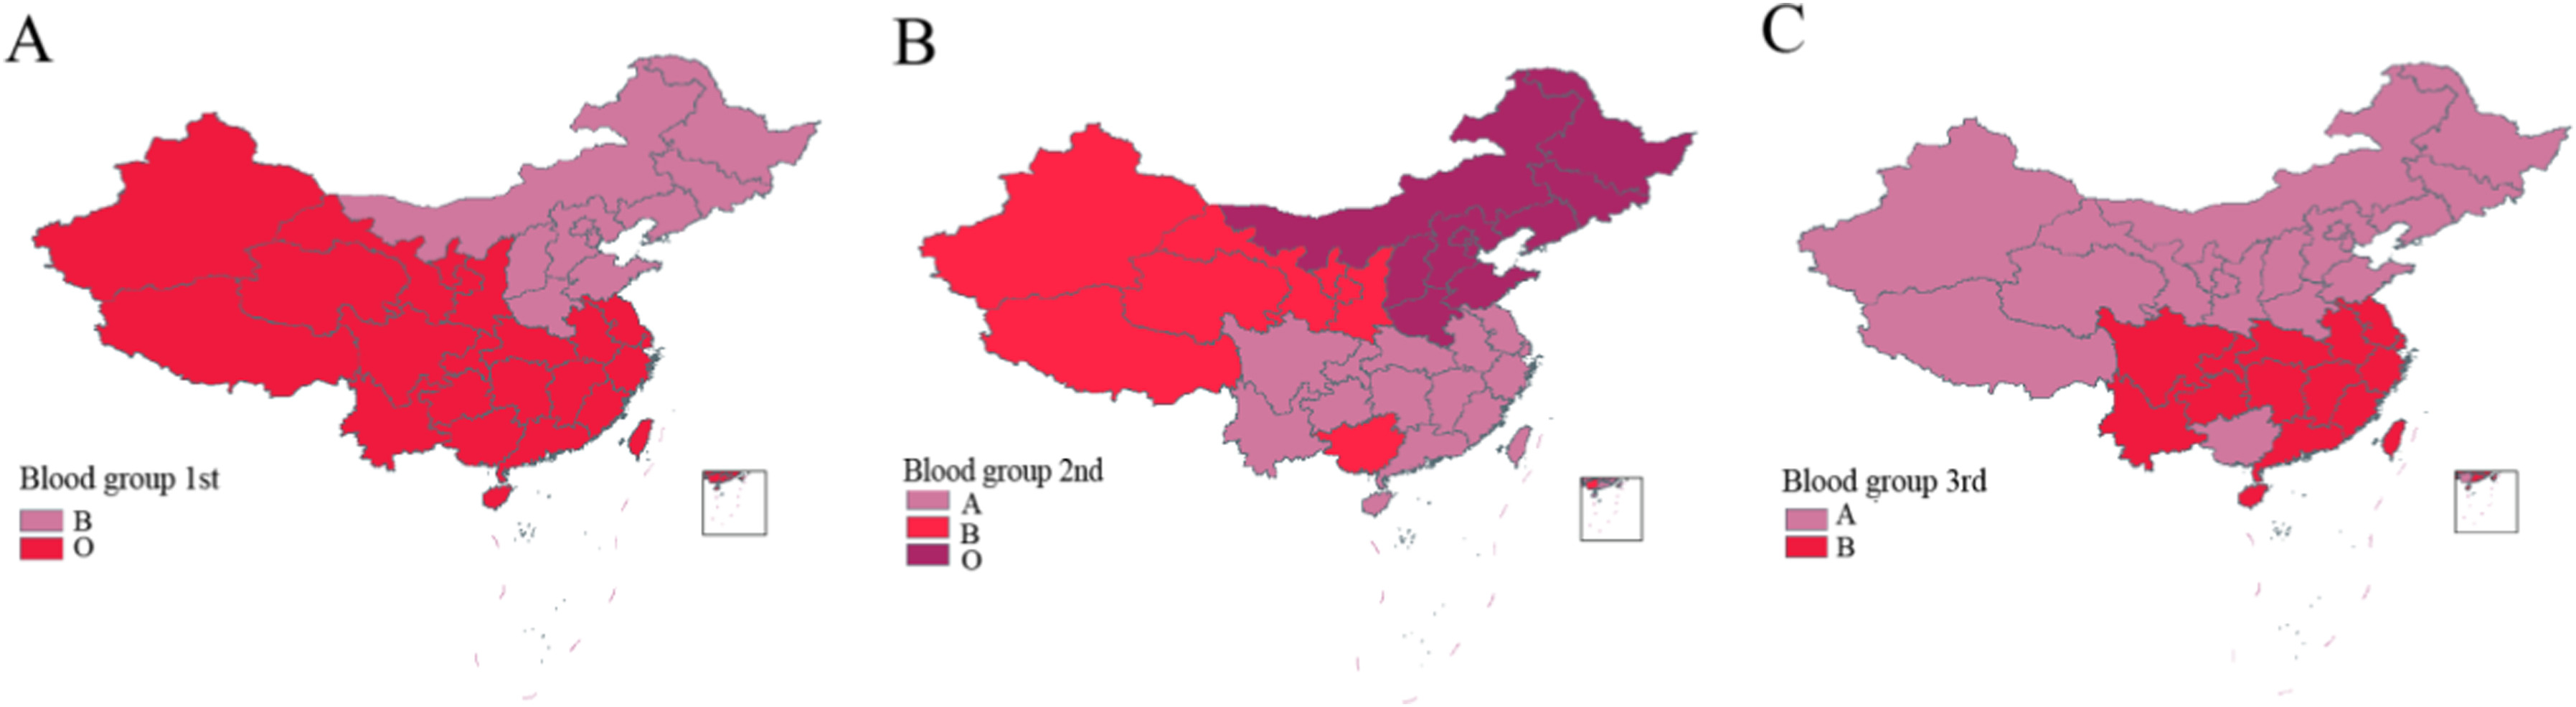
\includegraphics[width=350pt]{./img/Ranking of ABO blood group proportion in 34 provincial level of China.jpg}
        \caption{Ranking of ABO blood group proportion in 34 provincial level of China, 引用自\cite{WOS:000879413200018}}
        \label{fig:ChinaABO-1}
    \end{figure}

    \item 中国人ABO血型分布特征从北向南分为四个区:
    I区:B型为主,B、O、A趋向均衡;I区:O型为主,B型较低为23-26\%;皿区:O型为主为40-44\%,
    A与B接近,在23-28\%。IV区:0型38.74\%,B型33.64\%,A型20.62\%。(见图\ref{fig:ChinaABO-2})

    \begin{figure}[H]
        \centering
        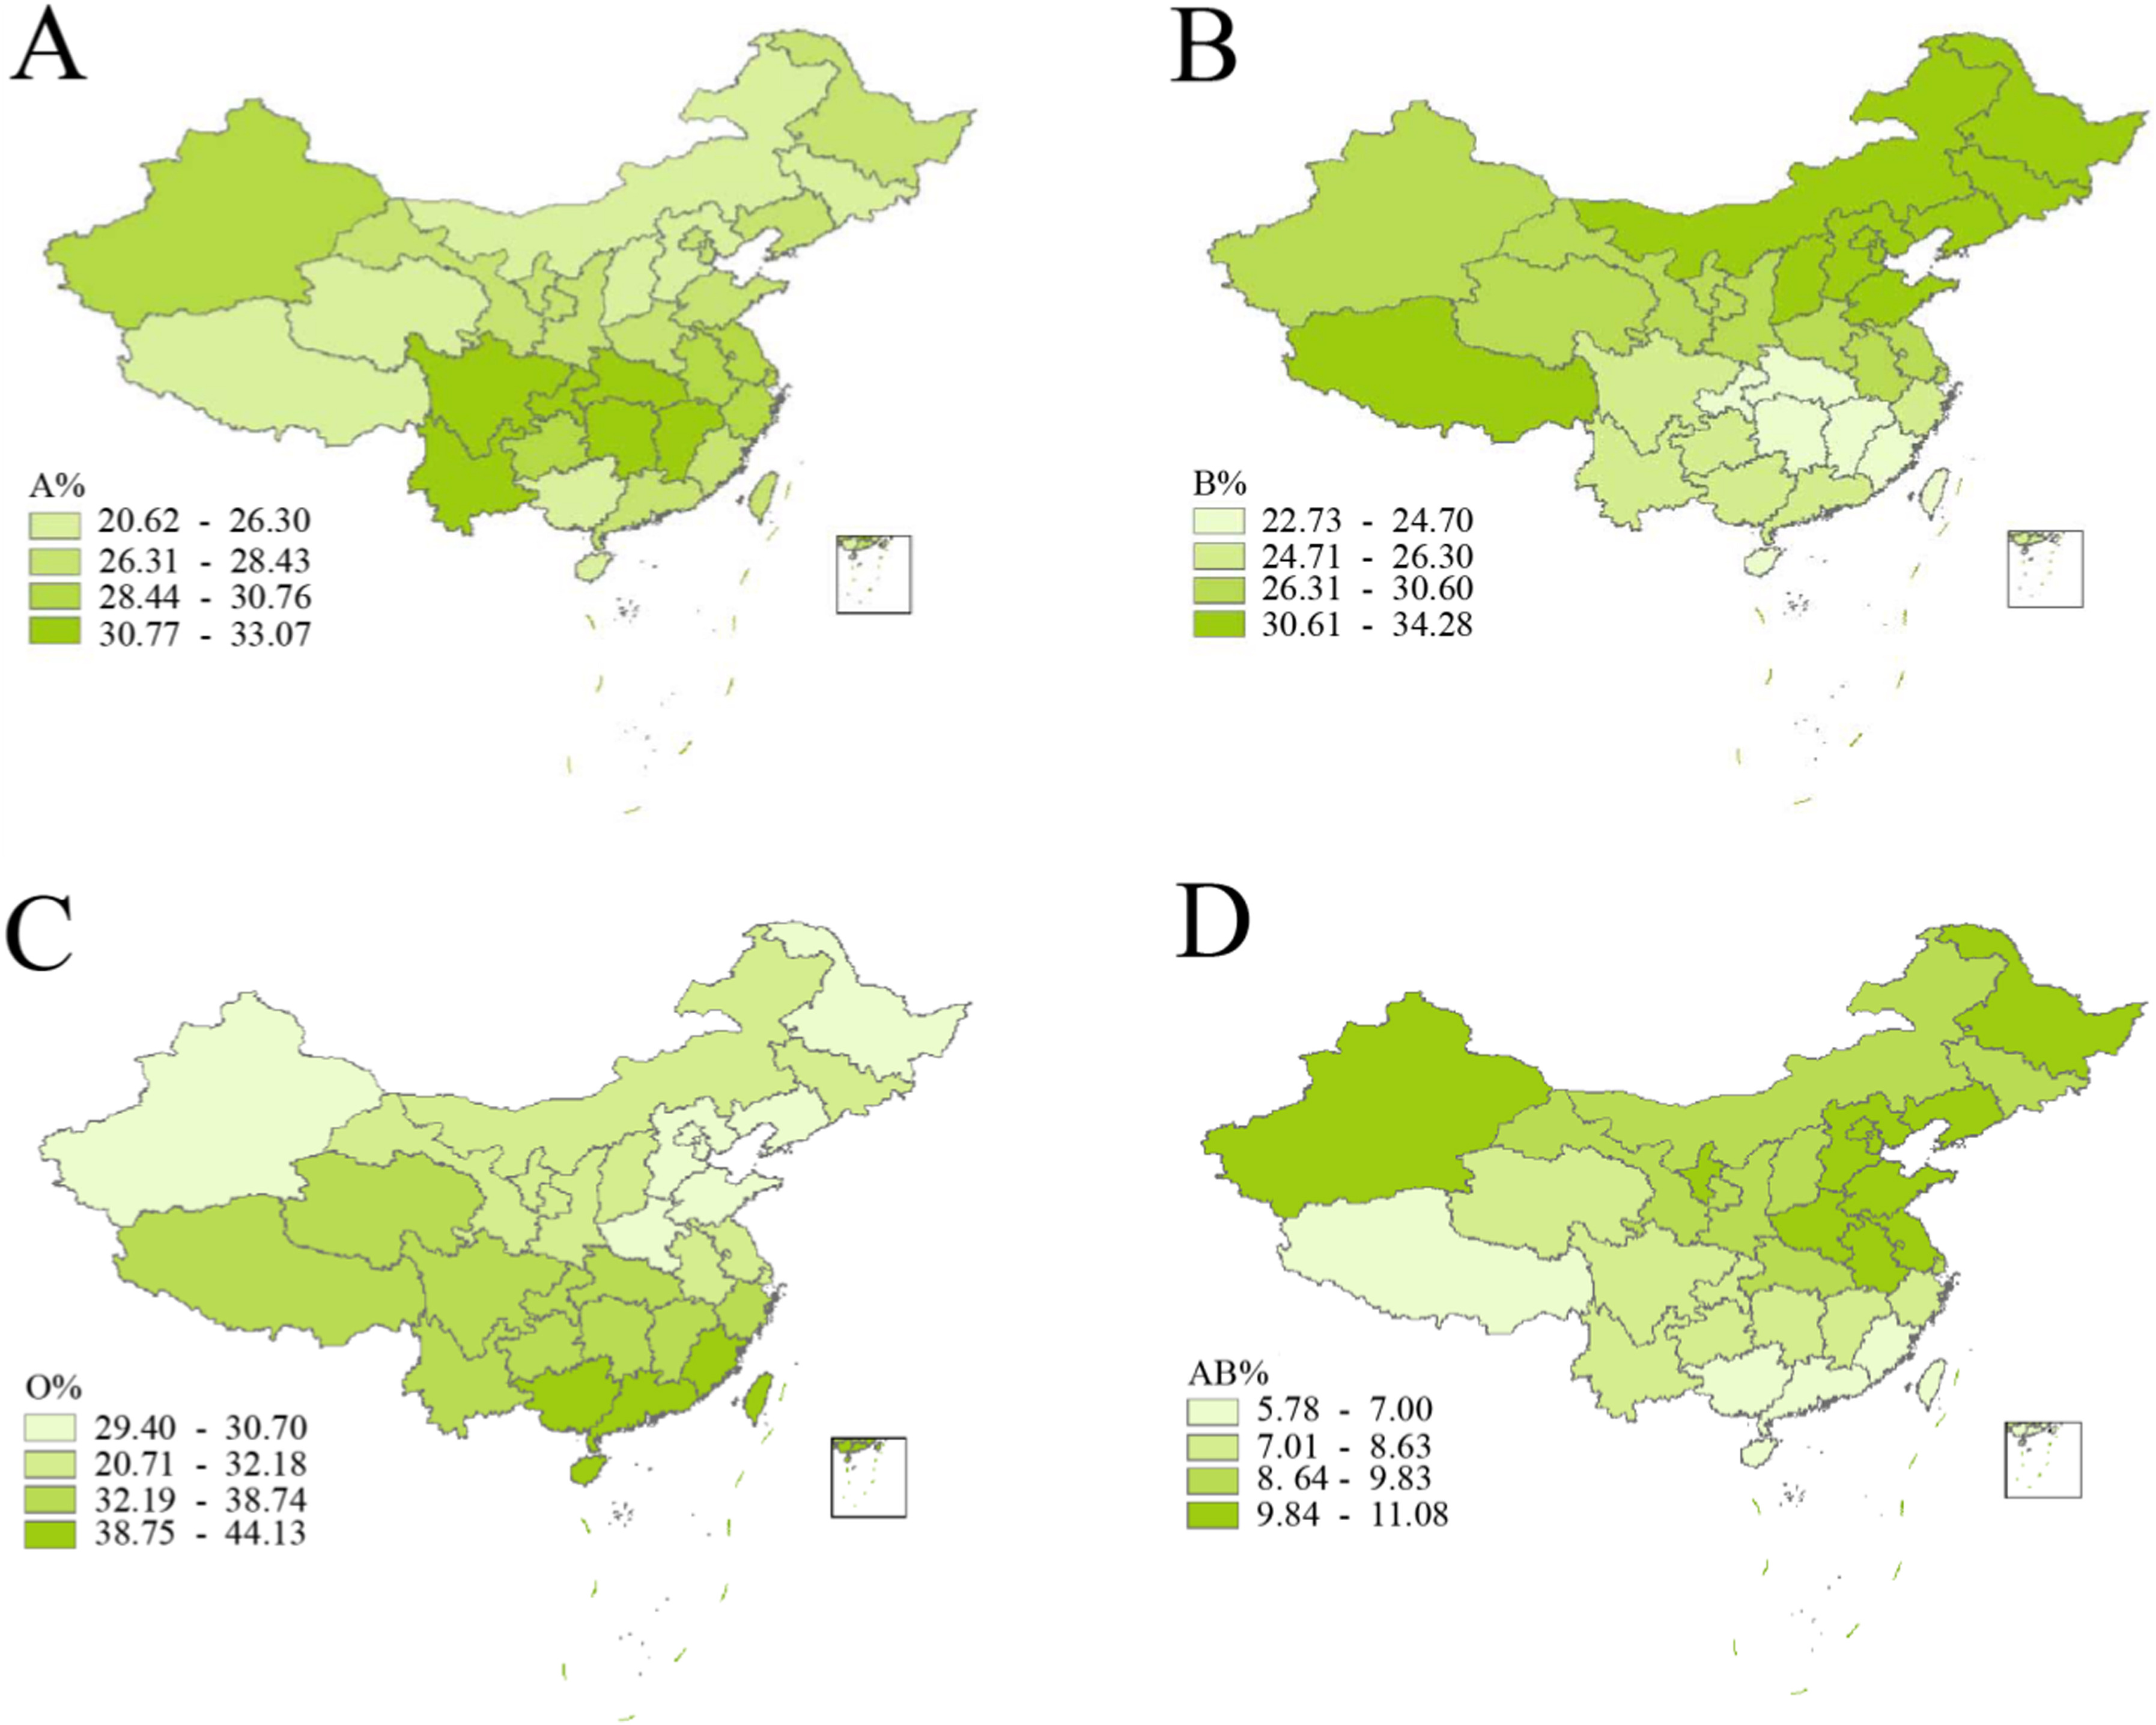
\includegraphics[width=350pt]{./img/The four ABO blood groups proportions in provincial-level distribution.jpg}
        \caption{The four ABO blood groups proportions in provincial-level distribution, 引用自\cite{WOS:000879413200018}}
        \label{fig:ChinaABO-2}
    \end{figure}

\begin{itemize}
    \item 人类ABO血型的群体遗传分析\par
\end{itemize}

人类ABO血型的群体遗传分析是遗传学中的一个经典实验,它是通过对群体中某一性状的调查分析,估算出该基因的等位基因频率和基因型频率,从而判断这个群体是否处于遗传平衡状态。\par
假定你所测试的群体是一个平衡群体。平衡群体的上下代之间等位基因频率和基因型频率保持不变,ABO血型的基因型、表型及其频率之间的关系式如下:

基因频率:  $$I^A=p, I^B=q, i=r$$

基因型频率:  $$I^AI^A=p^2,\,I^Ai=2pr,\,I^BI^B=q^2,\,I^Bi=2qr,\,I^AI^B=2pq,\,ii=r^2$$

由此可以推导出如下理论频率:   $$I^A: p=1-\sqrt{q^2+2qr+r^2}=1-\sqrt{B+O}$$
$$I^B: q=1-\sqrt{p^2+2pr+r^2}=1-\sqrt{A+O}$$
$$r=\sqrt{r^2}=\sqrt{O}$$

根据D矫正p, q, r: $$D=1-p-q-r$$
$$p=p(1+0.5D),\,q=q(1+0.5D),\,r=(r+0.5D)(1+0.5D)$$

理论表现型频率:  $$phenotypic\,frequency\,of\,A=p^2+2pr,\,phenotypic\,frequency\,of\,B=q^2+2qr$$
$$phenotypic\,frequency\,of\,AB=2pq,\,phenotypic\,frequency\,of\,O=r^2$$

通过基因频率来推算各种基因型频率的理论预期值,再与实际测试结果进行$x^2$检验。根据x值和自由度(n=2),查表(见附录九)。如果P>
0.05,差异不显著,说明测试值与理论值相符合,认为该群体为平衡群体;如果P<0.05,差异显著,说明测试值与理论值不符合,则认为该群体是不平衡群体。
也可以使用R语言进行计算,如代码\ref{lst:r-example}所示:

\begin{lstlisting}[language=R, caption={R示例}, label={lst:r-example}, style=myRstyle]
chisq.result <- chisq.test(x=c(A.data,B.data,AB.data, O.data), p=c(a.p,b.p,ab.p,o.p),rescale=T) # 默认自由度n-1
pchisq(chisq.result$statistic, df=2, lower.tail=F) # 更正自由度
\end{lstlisting}

\section{人类部分单基因体表性状及其遗传分析}
\subsection{体表性状}
人类的各种性状都由特定的基因控制形成。由于个体的遗传基础不同,某些特定的性状在不同的个体表现不同。通过对群体中某一性状的调查分析,可以估算出该基因的等位基因频率和基因型频率\cite{SWXT201802015}。系谱分析法常用于单基因遗传性状研究,本实验将调查一些已知的人体部分单基因性状,初步了解这些性状的遗传特性。在可能的情况下,学生对自己家族或别人家族的某些体表性状进行调查,画出系谱图,根据所测得的数据进行群体遗传结构分析,同时可判断这个群体是否处于遗传平衡状态。

\begin{longtable}{ccc|ccc}
    \toprule
    性状     & 显性   & 隐性  &  性状   & 显性   & 隐性  \\
    \midrule
    耳垂     & 耳垂   & 无耳垂  & 扣手指    & 右手扣  & 左手扣  \\
    卷舌     & 卷舌   & 平舌   & 眼睑     & 双眼睑  & 单眼睑  \\
    叠舌     & 非叠舌  & 叠舌   & 酒窝     & 有酒窝  & 无酒窝  \\
    美人尖    & 有美人尖 & 无美人尖 & 多指     & 有多指  & 无多指  \\
    拇指类型   & 直型   & 过伸指  & 白化症    & 正常   & 白化症  \\
    环食指长 & 食指长  & 食指短  & 红绿色盲   & 正常   & 红绿色盲 \\
    血友病   & 正常   & 血友病  & ...   & ...   & ...  \\
    \bottomrule
    \caption{人类部分单基体表性状}
\end{longtable}

\subsection{遗传分析}
假设某一基因位点上有一对等位基因A和a,它们在群体中出现的频率分别为p和q;基因型AA、Aa 和aa
在群体中出现的频率分别为D、H和R,如果这个群体(D,H,R) 是完全随机交配的,那么这一群体的基因型频率和等位基因频率的关系是:
$$D=p^2, H=2pq, R=q^2, D+H=p^2+2pq$$

无论一个基因位点上有几个等位基因,只要这个群体是随机交配的,等位基因频率就很难发生变化,物种就能保持相对的稳定,它们在群体中的遗传变化规律都遵循
Hardy-Weinberg 平衡定律。据此我们可以对人类群体进行等位基因频率的遗传分析。

\chapter{实验目的与方法}
\section{实验目的}
\begin{itemize}
    \item 通过人类部分单基因体表性状的调查分析,了解基因在群体水平上的传递规律\par
    \item 掌握遗传平衡群体基因频率和基因型频率的估算方法\par
    \item 进一步理解Hardy-Weinberg平衡定律,了解改变平衡的因素\par
\end{itemize}

\section{实验方法}
\subsection{实验材料与数据收集}
\begin{itemize}
    \item 实验数据\par
    兰州大学生命科学学院21级学生的微量血型

    \item 试剂\par
    \begin{itemize}
        \item 75\% 医用酒精\par
        \item 0.9\% 生理盐水\par
        \item 标准的抗A和抗B血清\par
    \end{itemize}

    \item 器具\par
    显微镜, 电子天平, 无菌采集针, 双凹载玻片, 镊子, 牙签, 微量加样枪...

\end{itemize}
\subsection{ABO血型的检测}
\begin{itemize}
    \item 准备生理盐水
    于离心管中加人300-500mL生理盐水,备用。
    \item 准备标准血清
    取一洁净的双凹载玻片(或普通载玻片),在两端上角用记号笔标注A和B,然后在相应位置分别滴加标准的抗A和抗B型血清各一滴。
    \item 采血
    用75\%酒精棉球消毒 受检者的手指或耳垂,待乙醇挥发后立即用无菌采血针刺破皮肤,弃去第一滴血,然后用无菌枪头吸取15~25wL
    血液加入离心管中,轻弹管壁制成5\%的血细胞悬液,同时受检者用无菌棉签止血。
    \item 凝集实验
    在玻片的两种标准血清中分别滴加1滴血细胞悬液(注意滴头不要触及标准血清),立即用不同的牙签分别搅拌使血细胞悬液和血清充分混匀。
    \item 检测
    在室温下每隔数分钟轻轻晃动玻片几次以加速凝集,过5~15
    min后观察,若混匀的血清由浑浊变为透明,并出现大小不等的红色颗粒,则表明红细胞已凝集;若仍呈泽浊状,不出现颗粒则无凝集;有时会出现疑似凝集,但稍微晃动玻片又呈浑浊状,则不属凝集。若观察不清可在低倍镜下观察。室温过低时可将玻片置于37°C恒温箱中,以促其凝集。
    \item 统计
    根据ABO血型检查结果,判断受检者的血型并统计。
\end{itemize}

\subsection{人类部分单基因性状的调查}
按照单基因体表性状的判定标准,观察并统计各种体表性状的变异类型在所调查人群中出现的频率。选择几个体表性状对自己家族或别人家族进行调查,画出相应的系谱图,确定该性状的遗传特性。

\chapter{研究结果与分析}
\section{ABO血型的群体遗传分析}
\subsection{ABO血型的检测结果}
\begin{longtable}{cccc}
    \toprule
    表现型 & 频数 \\
    \midrule
    A型 & 58 \\
    B型 & 61 \\
    O型 & 67 \\
    AB型 & 13 \\
    \bottomrule
    \caption{ABO血型的检测结果}
    \label{tbl:ABOcount}
\end{longtable}
\subsection{数据分析}
\begin{itemize}
    \item 计算表现型频率\par
    通过表\ref{tbl:ABOcount}中的数据,我们可以计算出各个血型的频率,如代码\ref{lst:abo-r-calcrawfrequency}所示。
    \begin{lstlisting}[caption={计算频率}, label={lst:abo-r-calcrawfrequency}, style=myRstyle]
    stu.num <- nrow(data)                     # Calculate the number of students
    abo.count <- table(data$ABO血型)      # Count occurrences of each blood type
    blood.count <- data.frame(
      count = c(abo.count["A"], abo.count["B"], abo.count["O"],
                abo.count["AB"]),
      frequency = c(abo.count["A"]/stu.num, abo.count["B"]/stu.num,
                    abo.count["O"]/stu.num, abo.count["AB"]/stu.num)
    )

    # Calculate frequencies
    p.raw <- 1 - sqrt(blood.count["A", 2] + blood.count["O", 2])
    q.raw <- 1 - sqrt(blood.count["B", 2] + blood.count["O", 2])
    r.raw <- sqrt(blood.count["O", 2])
    \end{lstlisting}
    \item 计算理论基因频率\par
    接下来我们可以计算出各个血型基因的频率并根据公式$D=1-p-q-r$计算纠正值D,如代码\ref{lst:abo-r-calcgenefrequency}所示。
    \begin{lstlisting}[caption={计算理论基因频率}, label={lst:abo-r-calcgenefrequency}, style=myRstyle]\

    # Calculate uncorrected frequencies and correction factor D
    p.raw <- 1 - sqrt(blood.count["A", 2] + blood.count["O", 2])
    q.raw <- 1 - sqrt(blood.count["B", 2] + blood.count["O", 2])
    r.raw <- sqrt(blood.count["O", 2])
    D <- 1 - p.raw - q.raw - r.raw
    \end{lstlisting}
    \item 通过纠正值D计算理论基因频率与基因型频率,如代码\ref{lst:abo-r-calccorrectgenefrequency}所示。
    \begin{lstlisting}[caption={通过纠正值D计算矫正理论基因频率}, label={lst:abo-r-calccorrectgenefrequency}, style=myRstyle]

    # Calculate corrected frequencies
    p <- p.raw * (1 + 0.5 * D)
    q <- q.raw * (1 + 0.5 * D)
    r <- (r.raw + 0.5 * D) * (1 + 0.5 * D)

    # Calculate phenotypic frequencies based on corrected frequencies
    blood.count <- data.frame(
      count = blood.count$count,
      frequency = blood.count$frequency,
      phenotypicfrequency = c(p^2 + 2*p*r, q^2 + 2*q*r, r^2, 2*p*q)
    )
    \end{lstlisting}
    \item 原始数据与矫正后的基因型频率卡方检验, 如代码\ref{lst:abo-r-chisqtest}所示。
    \begin{lstlisting}[caption={原始数据与矫正后的基因型频率卡方检验}, label={lst:abo-r-chisqtest}, style=myRstyle]

    # Perform chi-square test using observed counts and expected frequencies
    chisq.result <- chisq.test(
        x = object@blood.count$count,
        p = object@blood.count$phenotypicfrequency,
        rescale = TRUE)

    # Calculate p-value using the chi-square distribution
    p.value <- pchisq(chisq.result$statistic, df = 2,
                      lower.tail = FALSE)
    \end{lstlisting}
\end{itemize}
\subsection{结果与分析}
\begin{itemize}
    \item 结果如表\ref{tbl:ABOresult}所示
    \begin{longtable}{cccc}
        \toprule
        表现型 & 频数 & 频率 & 理论频率 \\
        \midrule
        A型 & 58 & 0.28431373 & 0.29708657 \\
        B型 & 61 & 0.29901961 & 0.28237099 \\
        O型 & 67 & 0.32843137 & 0.33006526 \\
        AB型 & 13 & 0.06372549 & 0.09047555 \\
        \bottomrule
        \caption{ABO血型的检测结果}
        \label{tbl:ABOresult}
    \end{longtable}

    P-value: 0.3965

    \item 分析\par
    根据统计, 在兰州大学21级生命科学学院的学生中, O心血的人数最多占32.84\%, A型血的人数次之占28.43\%, B型血的人数为29.90\%, AB型血的人数最少占6.37\%。
    这一结果与中国人群ABO血型分布情况(图\ref{fig:ChinaABO-1})非常相近, 说明我们的样本从一定程度上来说具有一定的代表性。

    P值为0.3965,大于0.05,差异不显著,说明测试值与理论值相符合,认为该群体为平衡群体。

\end{itemize}
\section{人类部分单基因体表性状的调查}
\subsection{调查结果}
\begin{longtable}{cccc}
    \toprule
    性状    & 表型1(计数)  & 表型2(计数)   \\
    \midrule
    性别 & 男 (115) & 女 (89) \\
    民族 & 汉族 (188) & 少数民族 (16) \\
    生源地 & 秦岭淮河以北 (126) & 秦岭淮河以南 (78) \\
    耳垂 & 无耳垂 (66) & 有耳垂 (138) \\
    舌型 & 卷舌 (149) & 直舌 (55) \\
    美人尖 & 无尖 (129) & 有尖 (75) \\
    拇指类型 & 过伸型 (87) & 直型 (117) \\
    环食指长 & 环指长 (156) & 食指长 (48) \\
    扣手 & 右手拇指在上 (94) & 左手拇指在上 (110) \\
    眼睑 & 单眼皮 (69) & 双眼皮 (135) \\
    酒窝 & 无 (146) & 有 (58) \\
    \bottomrule
    \caption{人类部分单基因性状的调查}
\end{longtable}

基因频率:

有耳垂: 0.6764706

卷舌: 0.1348039

有尖: 0.1838235

过伸型: 0.2867647

环食指长: 0.1176471

右手拇指在上: 0.2696078

双眼皮: 0.3308824

有酒窝: 0.1421569

\chapter{\texorpdfstring{讨 \quad 论}{讨论}}
\begin{enumerate}
    \item ABO血型的群体遗传分析结果:

    \begin{itemize}
        \item 由于我在开始分析的时候还有部分同学的血型数据没有填写, 所以我在分析的时候将这部分数据排除在外, 这一问题有可能会导致我的实验结果与他人有些微差距

        \item 在分析时我选用了表现型频率而不是基因型频率, 这是因为在实验中我们只能通过观察表现型来判断基因型, 所以我认为表现型频率更能反映实验结果

        \item 根据实验结果: A型血的频率为0.28431373, B型血的频率为0.29901961, O型血的频率为0.32843137, AB型血的频率为0.06372549。
    p值为0.3965, 大于0.05, 差异不显著, 说明测试值与理论值相符合, 认为该群体为平衡群体。这与我们的预期相符合, 因为我们的群体比较随机, 而且符合Hardy-Weinberg平衡定律满足的条件。

        \item  但是, 由于我们的样本量较小, 且我们的样本并不是完全随机的, 所以我们的实验结果可能会有一定的偏差, 但是这个偏差并不会很大。
    \end{itemize}

    \item 人类部分单基因性状的调查:
    
    \begin{itemize}
        \item 总结调查的人类部分单基因性状,包括耳垂、舌卷、眼睑等。

        \item 统计各性状在调查人群中的频率,并分析其遗传特性。
    \end{itemize}
    
    \item 卡方检验:
    
    \begin{itemize}
        \item 讨论卡方检验的结果, 包括统计显著性水平和p值。

        \item 解释卡方检验对于验证Hardy-Weinberg平衡的重要性。
    \end{itemize}
    
    \item 实验的局限性和改进方向:
    
    \begin{itemize}
        \item 局限性:
        
        样本容量的限制: 实验中使用的样本容量可能受到一定的限制,这可能导致对整个人群的遗传结构进行全面研究的难度。更大规模的样本可能更好地代表整体人群。

        地理和人口的差异: 实验中可能来自不同地区的群体数量不同, 例如来自甘肃的生源更多,这可能导致研究结果的局限性,因为不同地区或人群可能存在基因频率的差异。

        基因突变和漂变: 实验可能未考虑到基因突变和漂变等因素,这些因素可能对遗传平衡的研究产生影响。未来的研究可以更深入地考虑这些变异。

        \item 改进方向:
        
        增加样本规模: 扩大实验的样本规模,以更全面地代表目标人群。这可以通过增加受试者的数量或在更多地理区域招募受试者来实现。

        多样性考虑: 将实验范围扩大到包含不同族群和人口类型,以更好地理解遗传平衡在不同群体中的表现。这有助于提高研究的外部有效性。

        考虑基因变异: 对基因突变和漂变等因素进行更详细的研究,以更准确地了解基因频率的演变。这可以通过深入分析基因组数据来实现。

        引入更多单基因性状: 考虑引入更多的人类单基因性状,以便更全面地研究基因的传递规律。这有助于深入了解遗传平衡的细节。

        跨学科研究: 将遗传学与其他学科(例如人类学、地理学)相结合,以更全面地理解人群遗传结构和遗传平衡。这可以为研究提供更多的背景信息和深层次的解释。
    \end{itemize}
    
    \item 实验的意义和应用价值:
    
    \begin{itemize}
        \item 深入理解基因在群体水平上的传递规律: 通过对人类ABO血型和部分单基因性状的遗传分析,可以深入理解基因在群体中的传递规律。这有助于揭示群体遗传结构、基因频率以及基因型频率等重要信息,为进一步的遗传研究提供基础。

        \item 掌握遗传平衡群体基因频率和基因型频率的估算方法: 实验中涉及了使用Hardy-Weinberg平衡定律进行基因频率和基因型频率的估算。掌握这些估算方法有助于在研究不同群体的遗传特征时,对基因频率的变化进行预测和解释。

        \item 进一步理解Hardy-Weinberg平衡定律及其影响因素: 通过实验,研究者可以更深入地理解Hardy-Weinberg平衡定律,了解什么因素可能破坏平衡状态。这对于理解群体遗传动态、进化过程中的影响因素具有重要意义。

        \item 对人类群体遗传结构的认识: ABO血型和其他单基因性状的调查分析有助于了解人类群体的遗传结构,例如不同血型在特定群体中的分布情况。这对于医学、人类学等领域的研究具有重要的参考价值。

        \item 培养实验技能、科学思维和数据分析能力: 通过进行实验,能够培养实验操作技能,学会运用遗传学原理进行实际研究。同时,对实验结果进行数据分析和解释,培养了科学思维和数据分析能力,为将来从事科研工作奠定基础。
    \end{itemize}
\end{enumerate}

%论文后部
\backmatter


%=======%
%引入参考文献文件
%=======%
\bibdatabase{bib/database}%bib文件名称 仅修改bib/ 后部分
\printbib
\nocite{*} %显示数据库中有的,但是正文没有引用的文献



\Appendix

本文相关的分析数据,代码以及latex文件请见附件(\href{https://github.com/zehua0417/GeneticExperimentReport/tree/main/2_Genetic%20Analysis%20and%20Correction%20of%20Human%20ABO%20Blood%20Types%20and%20Some%20Monogenic%20Traits}{点我打开链接})

%\Thanks


%\Grade %这一句才是成绩页,上面是填写


\end{document}
